\subsubsection{Meal schedule} \label{MealScheduleSketches}
The two figures in this section, \cref{MealScheduleList} and \cref{MealScheduleBar}, displays two design ideas for the meal schedule. The two ideas both have a weekly and a daily overview. The weekly overview gives the user a quick view of planned meals with little but relevant information. Whereas the daily overview gives the user a specific and detailed overview of specific recipes on a day.

\begin{figure}[H]
	\centering
    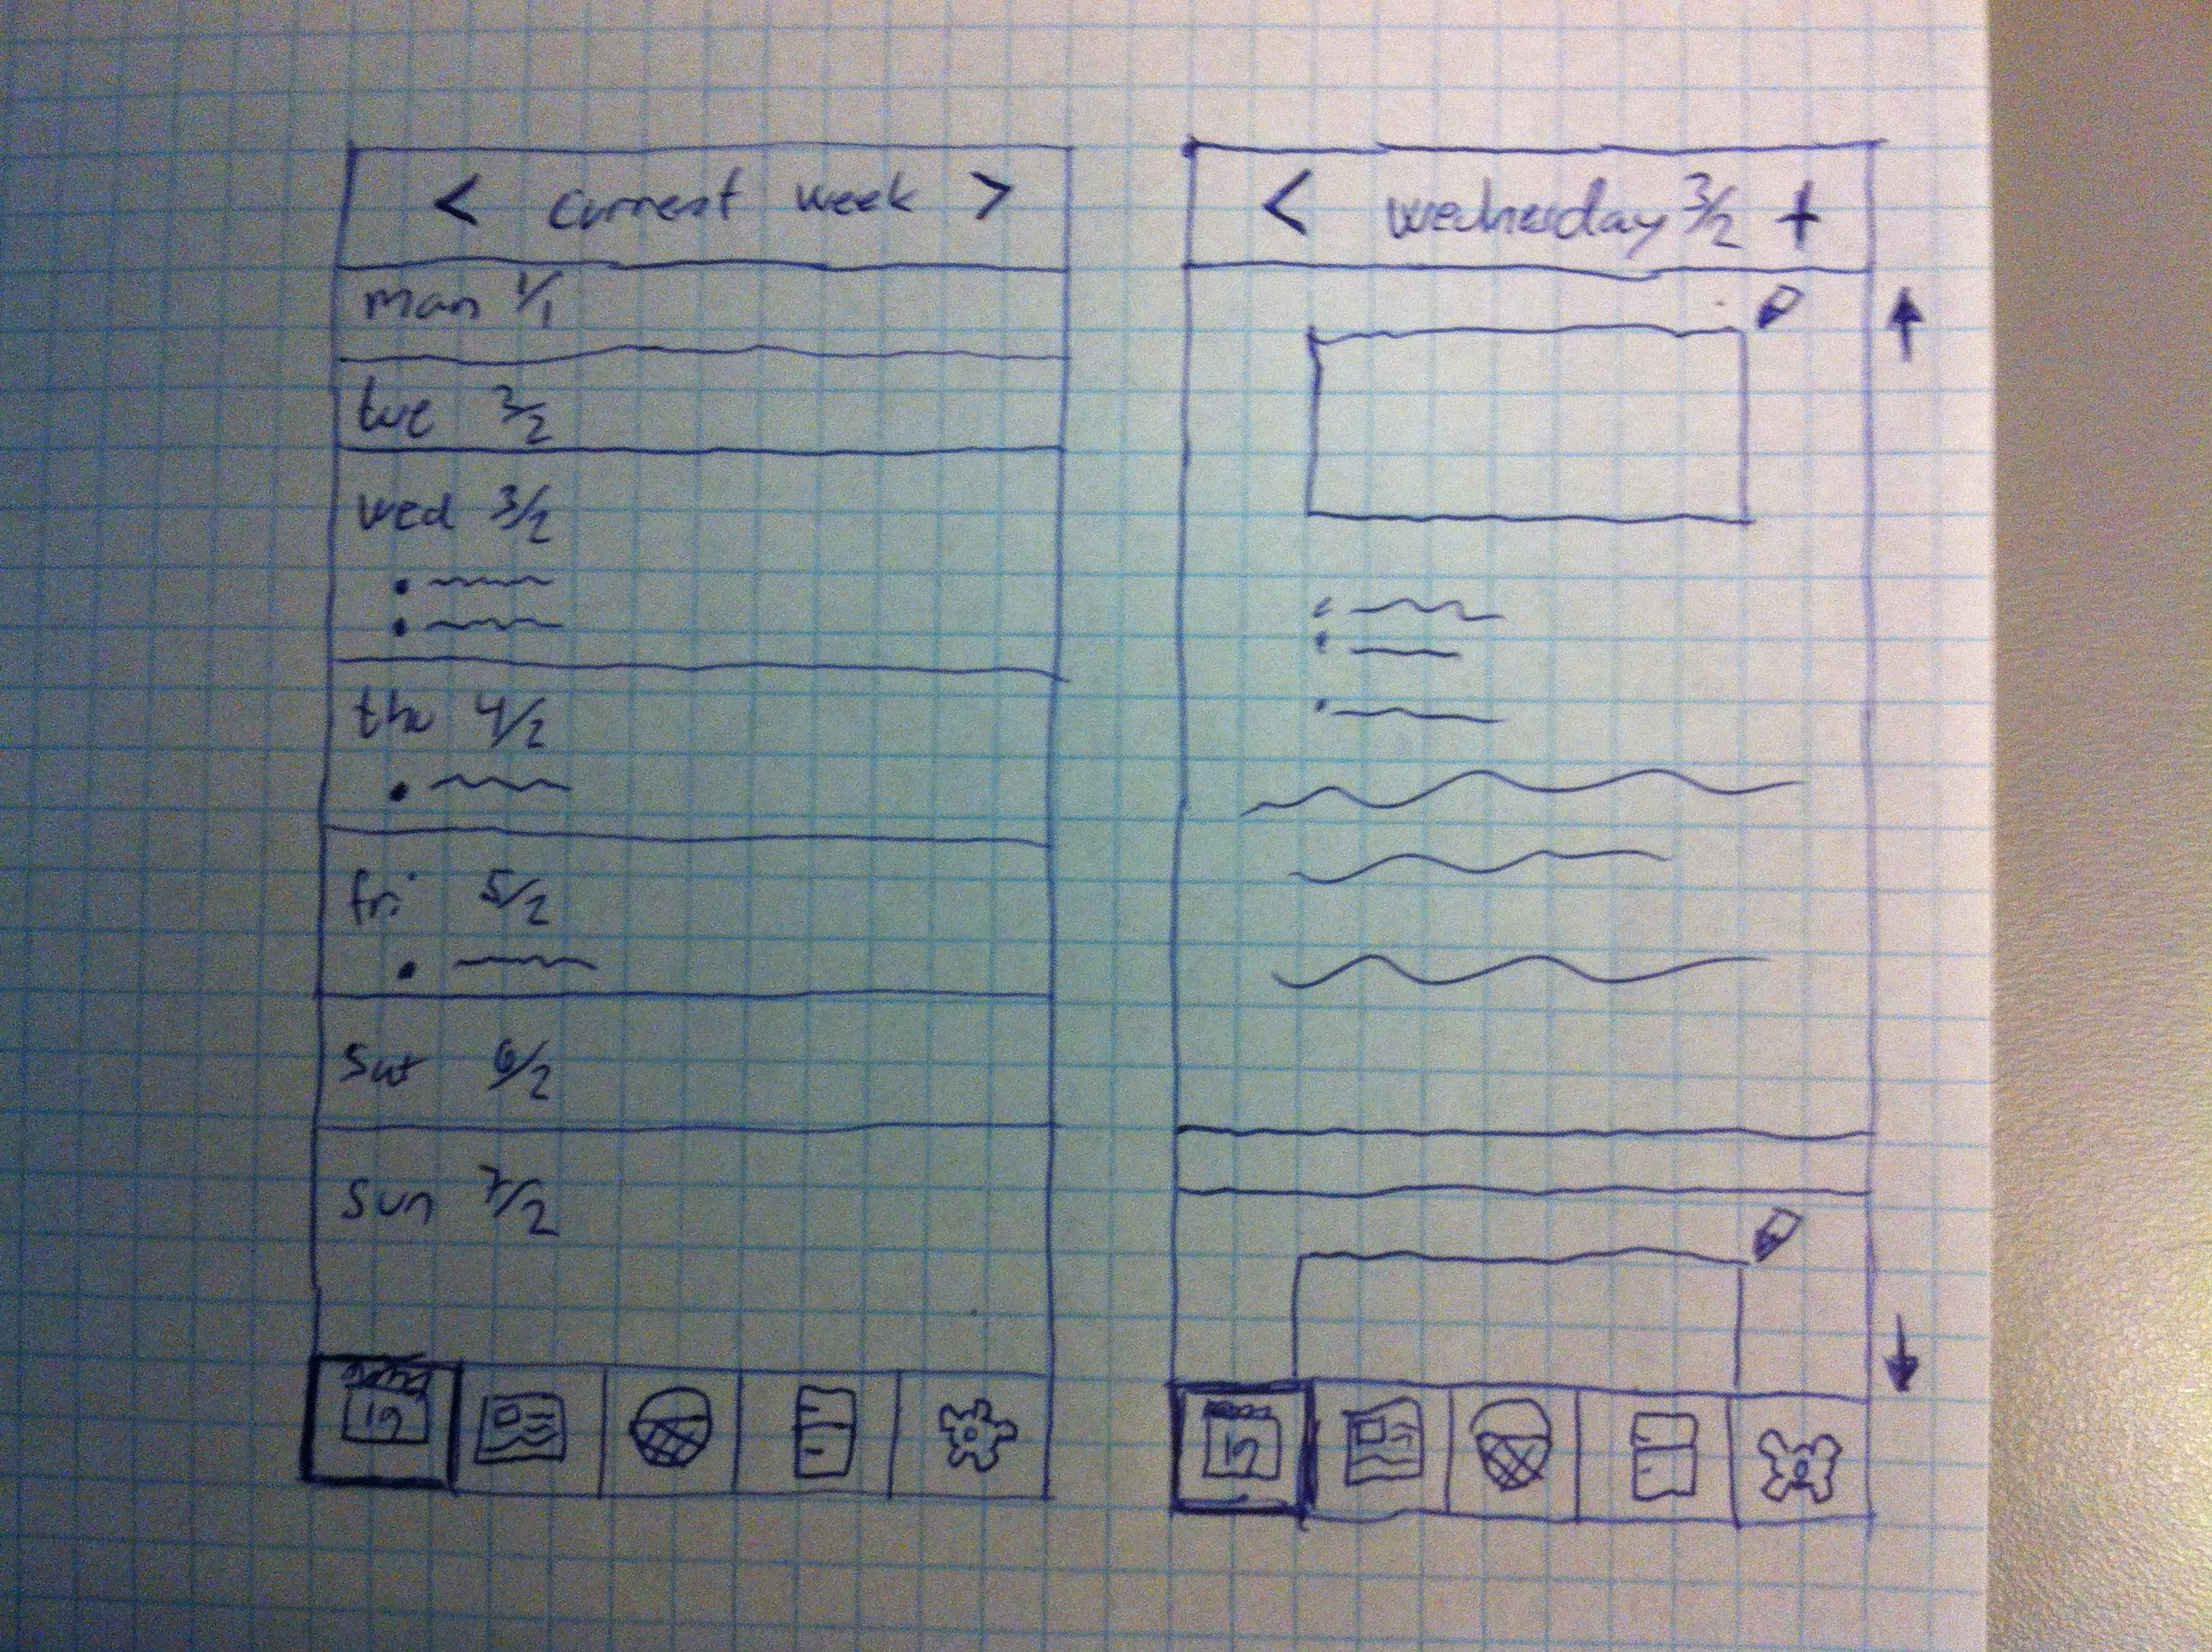
\includegraphics[width=0.5\textwidth]{Grafik/FoodPlanner/FinalMealScheduleSketch1}
	\caption{The left screen shows a specific week and the right screen shows scheduled meals on a specific day.}
	\label{MealScheduleList}
\end{figure}

\textbf{Two screen idea:} On \cref{MealScheduleList} two sketches are shown. They indicate the first idea that were thought of for the meal schedule design. The left sketch shows the meal schedule for a week, and the right shows the meals scheduled on a specific day.

Looking at the week schedule (the left sketch on \cref{MealScheduleList}) there are two elements to look at:

\begin{itemize}
    \item Top navigation bar
    \item Schedule
\end{itemize}

The top navigation bar is used to browse between different weeks. The bar has two navigation buttons and a text block with the currently selected week. The bottom and the top of the screen in mobile applications are often used to navigate. It is because of this that the top navigation bar is placed where it is. The position also has good symmetry with the bottom bar.

The schedule element of the sketch, shows a week of the schedule. The possibility to plan a week ahead is useful if the user plans the same day each week. Each day of the schedule would show the name of the recipe scheduled, the date of the day, and some of the ingredients needed in the recipe. If the user chooses to click a day, the screen would change to the right sketch on \cref{MealScheduleList}, and more information about the scheduled meals would appear.

Looking at the specific recipe (the right sketch on \cref{MealScheduleList}) there are two elements to look at:   

\begin{itemize}
    \item Navigation bar
    \item Scheduled recipes
\end{itemize}

The placement of the navigation bar has not changed. Its functionality has changed to suit the new screen. The bar has a button on the left side shaped as an arrow allowing the user to navigate back to the week schedule. Next to the arrow there are a text block displaying the chosen day e.g. Wednesday 3/2. The last element is a plus icon which allows the user to add recipes to the specific day.  

The right screen on \Cref{MealScheduleList} shows a list of all the recipes scheduled for a specific day. The list is ordered in a downwards fashion, so the user can go through all the scheduled recipes by scrolling through. If the user either want to change the recipe, or delete it, the user can click on the pencil icon, which means edit. A recipe consists of all the information about a recipe, this means picture, ingredients list and the list of instructions.

\begin{figure}[H]
	\centering
    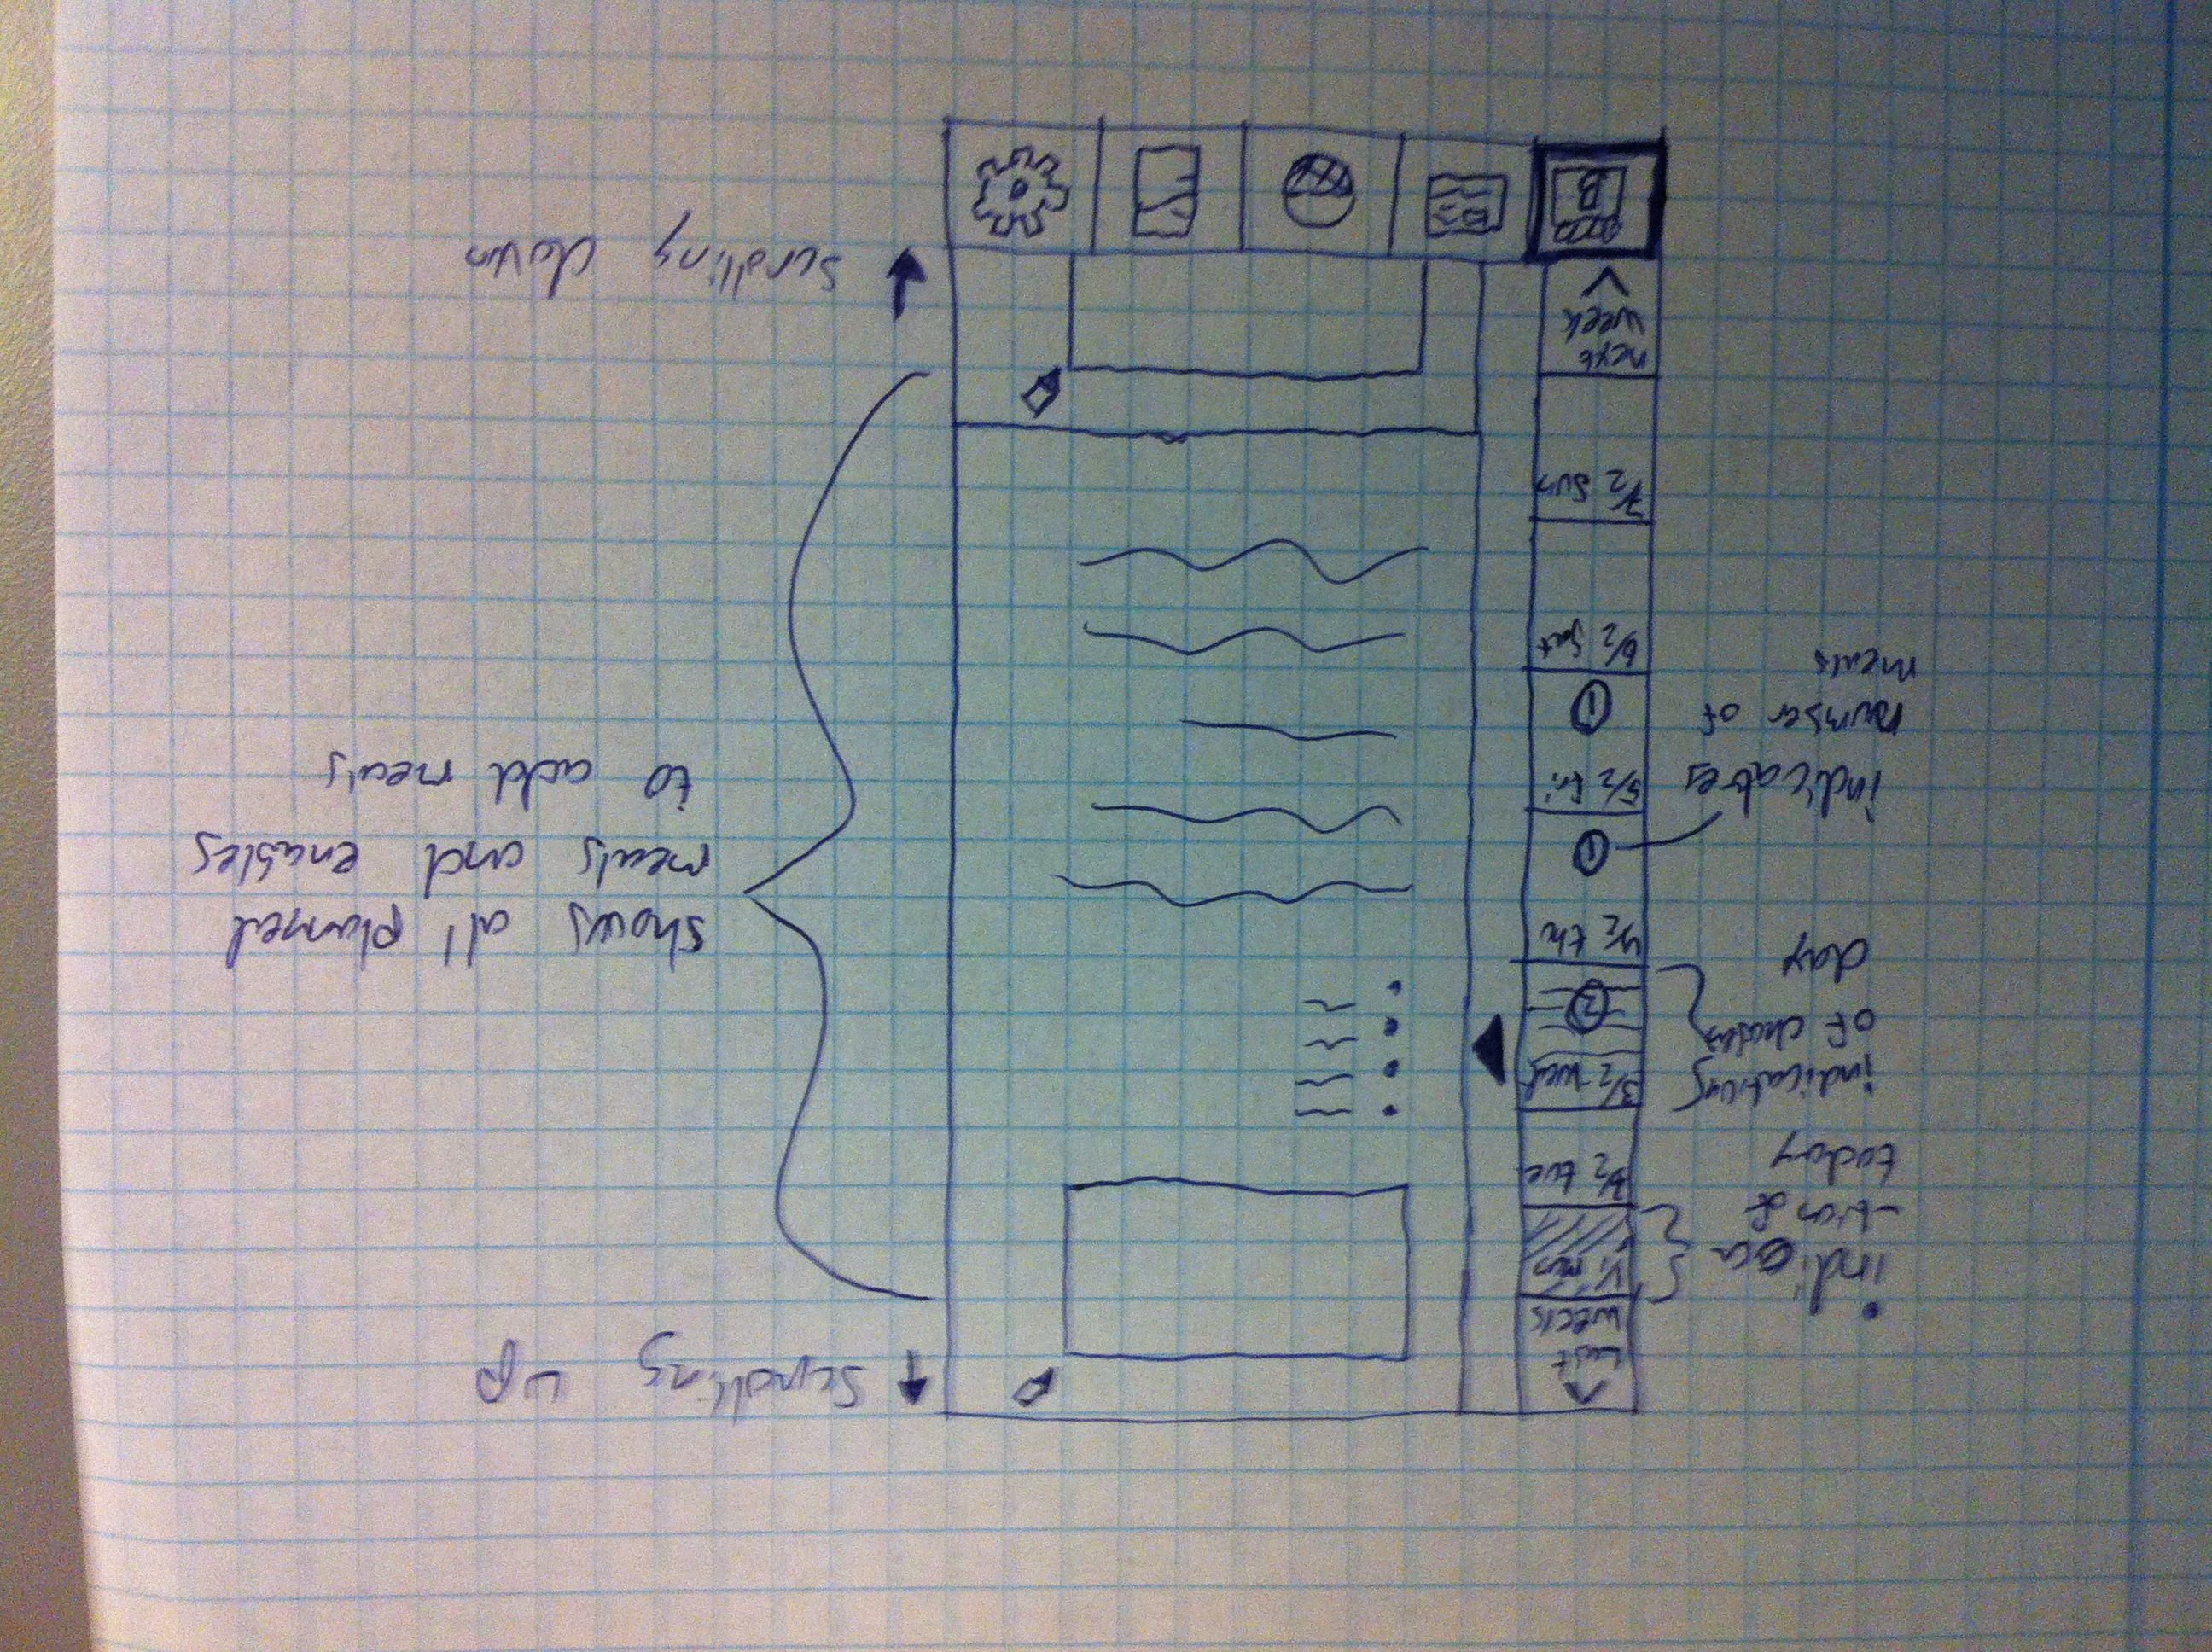
\includegraphics[width=0.5\textwidth]{Grafik/FoodPlanner/FinalMealScheduleSketch2}
	\caption{This sketch merges both of the screens sketched on \cref{MealScheduleList} into one screen with the weeks on the left bar and the scheduled meals as a list on the right side of the screen.}
	\label{MealScheduleBar}
\end{figure}

\textbf{Combined screen idea:} In \cref{MealScheduleBar} another design idea is envisioned. This idea has the weekly overview and the meals scheduled for a specific day combined in one window.

This design idea is used as a concept for the program's meal schedule design. The screen consists of two elements: 

\begin{itemize}
    \item Week navigation
    \item Scheduled recipes.
\end{itemize}

The week navigation is placed as a bar, in the left edge of the screen. This bar shows 7 days at a time, and have arrows going up and down to go browse between weeks. The reason for arrows and not the scrolling, is that by clicking a day, the scheduled recipes shown will change, so it is easy to misclick, if scrolling by swiping up and down is done, therefore buttons are used. The icons of the week navigation show the date, and a number. The number indicates the amount of recipes scheduled on the day, if no meals are scheduled, no number will be shown. 

The scheduled recipes element, works like the right screen on \cref{MealScheduleList} as described in the Meal schedule section.
